\documentclass[10pt, aspectratio=169]{beamer}

% --- Configuración de Tema Minimalista ---
\usetheme{metropolis}
\setbeamertemplate{section in toc}[sections numbered]
\setbeamercolor{background canvas}{bg=white}

% --- Paquetes ---
\usepackage[spanish]{babel}
\usepackage[utf8]{inputenc}
\usepackage{amsmath}
\usepackage{amsfonts}
\usepackage{amssymb}
\usepackage{graphicx}
\usepackage{siunitx} % Para unidades como \qty{200}{\milli\meter}
\usepackage{booktabs}

\usepackage{listings}
\usepackage{xcolor}

\lstset{
	language=Python,
	basicstyle=\ttfamily\tiny,
	keywordstyle=\color{blue},
	commentstyle=\color{gray},
	stringstyle=\color{orange},
	breaklines=true,
	frame=single
}

% --- Información de Portada ---
\title{Cinemática de Robots: Trayectoria más rápida}
\subtitle{Análisis Cinematográfico del Robot ABB IRB 140}
\author{Marco Brischetto, Ignacio Cavicchioli, Manuel Hirsch}
\institute{Facultad de Ingeniería, Universidad de Buenos Aires \\ 86.15 Robótica Industrial}
\date{Grupo: Droideka}
%\titlegraphic{\hfill\includegraphics[height=1cm]{logo_fiuba.png}} % Descomentar si tenés el logo

\begin{document}

	% --- Diapositiva 1: Portada ---
	\begin{frame}
		\titlepage
	\end{frame}

	% --- Diapositiva 2: El Problema ---
	\begin{frame}{El Problema: Optimización de Tiempo}
		\begin{itemize}
			\item \textbf{Objetivo:} Encontrar la trayectoria rectilínea de $\qty{200}{\milli\meter}$ que se recorra en el menor tiempo posible.
			\item \textbf{Restricción:} Velocidad cartesiana constante durante todo el recorrido.
			\item \textbf{Plataforma:} Robot industrial ABB IRB 140.
		\end{itemize}

		\begin{figure}
			\centering
			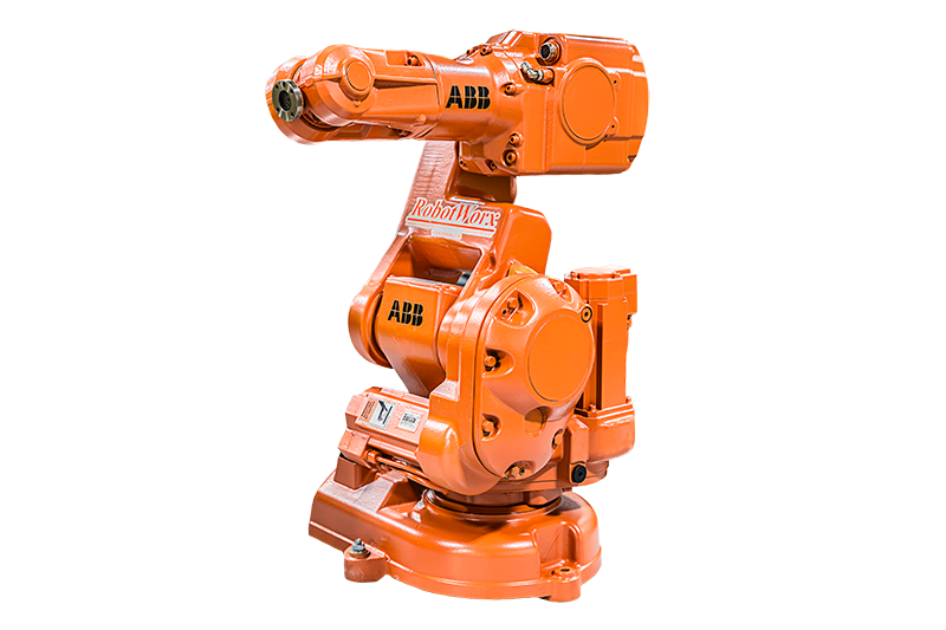
\includegraphics[width=0.5\textwidth]{ABB_IRB_140.png}
			\caption{IRB 140.}
		\end{figure}
	\end{frame}

	% --- Diapositiva 3: Simplificaciones para el Análisis ---
	\begin{frame}{Simplificaciones para el Análisis}
		Para abordar la complejidad del espacio de trabajo, definimos:
		\vspace{0.3cm}
		\begin{columns}
			\begin{column}{0.6\textwidth}
				\begin{itemize}
					\item \textbf{Reducción a 3 GDL:} Se analiza únicamente la traslación de la muñeca (primeros tres ejes).
					\item \textbf{Simetría:} Búsqueda en el plano $XZ$ (aprovechando simetría del robot).
					\item \textbf{Trayectorias:} Comparación entre movimientos paralelos a los ejes $Y$ (Horizontales) y $Z$ (Verticales).
				\end{itemize}
			\end{column}

			\begin{column}{0.4\textwidth}
				\begin{figure}
					\centering
					
\includegraphics[width=\textwidth]{"../memoria de proyecto/img/trayectorias.png"}
					\caption{Esquema de simplificación.}
				\end{figure}
			\end{column}
		\end{columns}
	\end{frame}


	% --- Diapositiva 4: Metodología: Grid Search ---
	\begin{frame}{Metodología: Búsqueda por Grilla (Grid Search)}
		\begin{itemize}
			\item Discretización del plano $XZ$ en una grilla de puntos de inicio potenciales.
			\item Evaluación de cada trayectoria mediante un algoritmo iterativo.
		\end{itemize}

		\begin{figure}
			\centering
			% Recordá ajustar la ruta si la imagen está en la carpeta de la memoria
			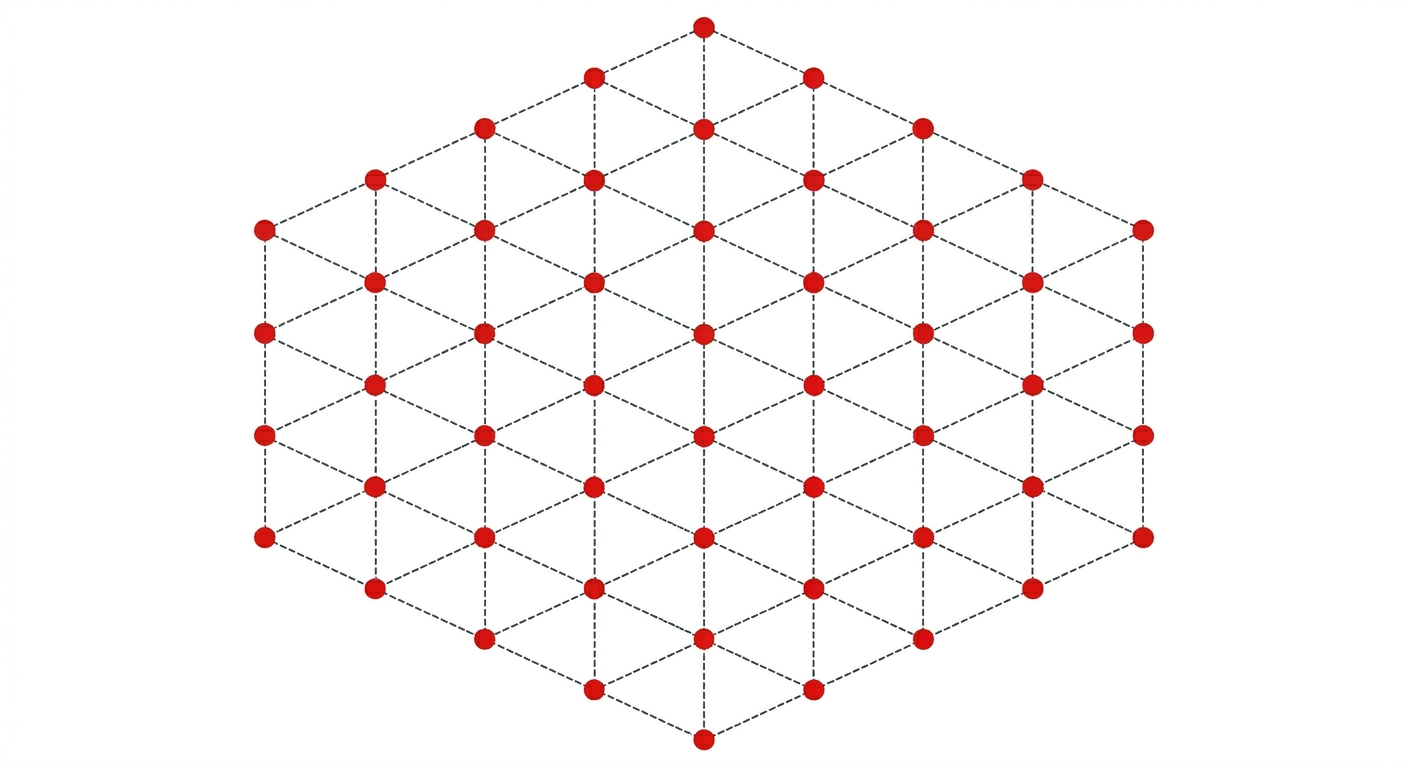
\includegraphics[width=0.6\textwidth]{grilla.png}
			\caption{Espacio de búsqueda discretizado para localizar el óptimo.}
		\end{figure}
	\end{frame}

	% --- Diapositiva 5: Metodología: El Cuello de Botella ---
	\begin{frame}{Cálculo del Cuello de Botella Cinemático}
		La velocidad máxima de la trayectoria está limitada por el eje que primero alcanza su límite operacional:

		\begin{equation*}
			\dot{q} = J^{-1} \cdot \dot{x}
		\end{equation*}

		\vspace{0.5cm}
		\begin{itemize}
			\item Se calcula la matriz \textbf{Jacobiana inversa} en cada punto de la recta.
			\item Se normaliza la velocidad cartesiana para que ninguna velocidad articular $\dot{q}_i$ supere su máximo de \textit{datasheet}.
			\item \textbf{Resultado:} La velocidad permitida para la trayectoria es el valor mínimo hallado en todo el recorrido.
		\end{itemize}
	\end{frame}

	% --- Diapositiva 6: Resultados Horizontales ---
	\begin{frame}{Resultados: Trayectorias Horizontales (Eje Y)}
		\begin{columns}
			\begin{column}{0.5\textwidth}
				\begin{itemize}
					\item \textbf{Velocidad máxima teórica:} $\qty{2.7}{\meter\per\second}$.
					\item El óptimo se encuentra con el brazo extendido y cerca de la base.
					\item Trayectoria: $(\qty{775}{\milli\meter}, \qty{-100}{\milli\meter}, \qty{131}{\milli\meter}) \to (\qty{775}{\milli\meter}, \qty{100}{\milli\meter}, \qty{131}{\milli\meter})$.
					\item El primer eje (rotación de la base) es el que aporta el mayor componente de velocidad lineal.
				\end{itemize}
			\end{column}
			\begin{column}{0.5\textwidth}
				\begin{figure}
					\centering
					% Cambiá el nombre por el de tu mapa de calor real
					
\includegraphics[width=\textwidth]{"../memoria de proyecto/img/mapa_calor_xz.png"}
					\caption{Distribución de velocidades máximas (Tray. Horizontales).}
				\end{figure}
			\end{column}
		\end{columns}
	\end{frame}


	% --- Diapositiva 7: Resultados Verticales ---
	\begin{frame}{Resultados: Trayectorias Verticales (Eje Z)}
		\begin{columns}
			\begin{column}{0.5\textwidth}
				\begin{itemize}
					\item \textbf{Velocidad máxima teórica:} $\qty{2.25}{\meter\per\second}$.
					\item Trayectoria: centrada en $(\qty{675}{\milli\meter}, \qty{0}{\milli\meter}, \qty{-125}{\milli\meter})$.
					\item Menor rendimiento general comparado con las trayectorias horizontales.
					\item Las articulaciones involucradas (hombro y codo) se saturan más rápido al intentar un avance puramente vertical.
				\end{itemize}
			\end{column}
			\begin{column}{0.5\textwidth}
				\begin{figure}
					\centering
					% Cambiá el nombre por el de tu mapa de calor real
					
\includegraphics[width=\textwidth]{"../memoria de proyecto/img/mapa_calor_verticales.png"}
					\caption{Distribución de velocidades máximas (Tray. Verticales).}
				\end{figure}
			\end{column}
		\end{columns}
	\end{frame}

	% --- Diapositiva 8: Validación en RobotStudio ---
	\begin{frame}{Validación en Entorno Virtual (RobotStudio)}
		\begin{itemize}
			\item Simulación de la trayectoria óptima en el controlador virtual de ABB.
			\item Verificación de que los 6 ejes operan dentro de los rangos seguros sin singularidades.
		\end{itemize}

		\vspace{0.2cm}
		\begin{figure}
			\centering
			% Cambiá el nombre por la captura de RobotStudio que tengan
			
\includegraphics[width=0.6\textwidth]{"../memoria de proyecto/img/robot img horizontal.png"}
			\caption{Validación de la trayectoria.}
		\end{figure}
	\end{frame}

	% --- Diapositiva 9: Análisis de Velocidad y Posición ---
	\begin{frame}{Análisis de Trayectoria Horizontal: Velocidad y Posición}
		\begin{columns}
			\begin{column}{0.5\textwidth}
				\begin{itemize}
					\item \textbf{Perfil de velocidad:} Incremento inicial seguido de una caída inesperada.
					\item \textbf{Efecto de ralentización:} El robot frena en zonas intermedias del recorrido.
					\item \textbf{Cercanía a singularidades:} Zonas donde la configuración del brazo exige movimientos bruscos.
				\end{itemize}
			\end{column}

			\begin{column}{0.5\textwidth}
				\begin{figure}
					\centering
					% Reemplaza por tus nombres de archivo reales
					
\includegraphics[width=0.7\textwidth]{"../memoria de proyecto/img/Y vs t y velocidad.png"}
					\caption{Gráficos de posición y velocidad vs. tiempo.}
				\end{figure}
			\end{column}
		\end{columns}
	\end{frame}

	% --- Diapositiva 10: Limitaciones del Entorno Real ---
	\begin{frame}{Discrepancias: Modelo (3 GDL) vs. Realidad (6 GDL)}
		\begin{block}{¿Por qué disminuye la velocidad en la simulación?}
			\begin{itemize}
				\item \textbf{Orientación obligatoria:} Imposibilidad de definir traslación pura $(x,y,z)$ sin considerar la rotación de la herramienta.
				\item \textbf{Acople de ejes:} Los 6 ejes deben trabajar en conjunto; la muñeca limita a los ejes principales.
				\item \textbf{Restricción del controlador:} El entorno de programación no permite aislar los primeros 3 ejes.
			\end{itemize}
		\end{block}

		\vspace{0.3cm}
		\begin{itemize}
			\item \textbf{Validez del cálculo:} Los resultados numéricos siguen siendo válidos como techo teórico del sistema.
			\item \textbf{Conclusión técnica:} El agregado de los 3 ejes extra y la dinámica real imponen las restricciones observadas.
		\end{itemize}
	\end{frame}




	% --- Horizontal ---
	\begin{frame}{Movimiento Vertical}
		\centering
		\href{https://drive.google.com/file/d/1GM2blQ1xi5XzenOf_VVzfB6owfeFwqe5/preview}{
			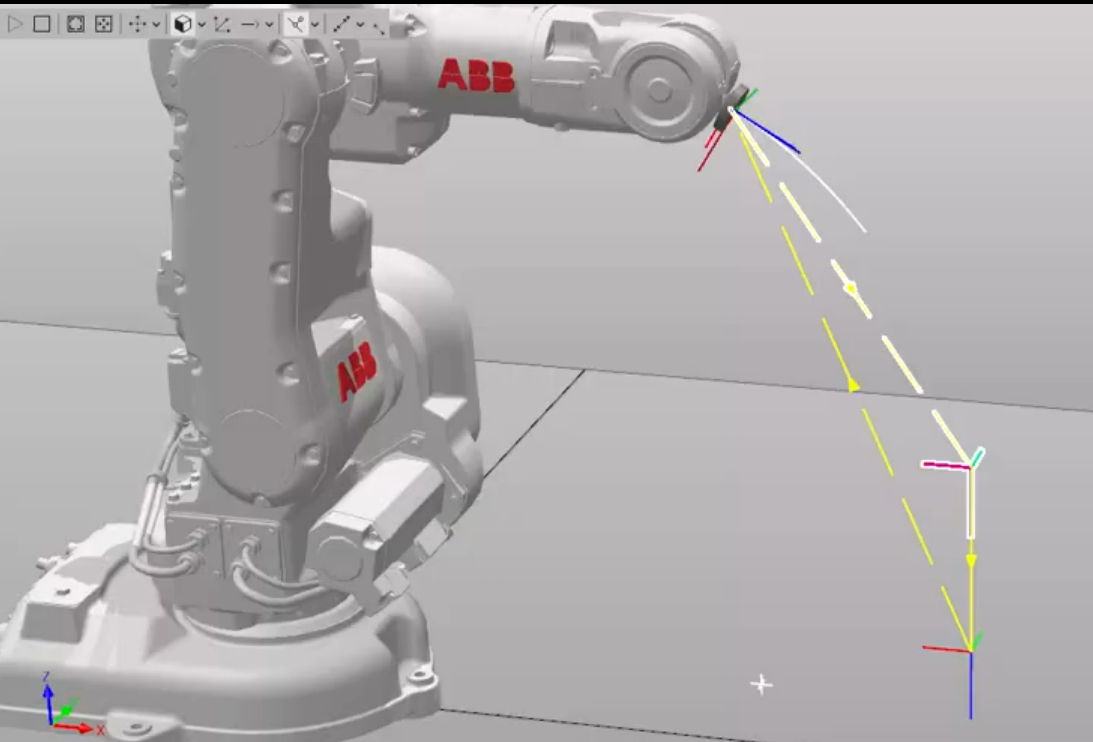
\includegraphics[height=0.75\textheight]{thumbnailver.png}
		}

		\vspace{0.5em}
		\small Click para reproducir el video
	\end{frame}

	% --- Vertical ---
	\begin{frame}{Movimiento Horizontal}
		\centering
		\href{https://drive.google.com/file/d/1BgFcqh8RINC6lT11EEQPpcjW3b-uaXks/preview}{
			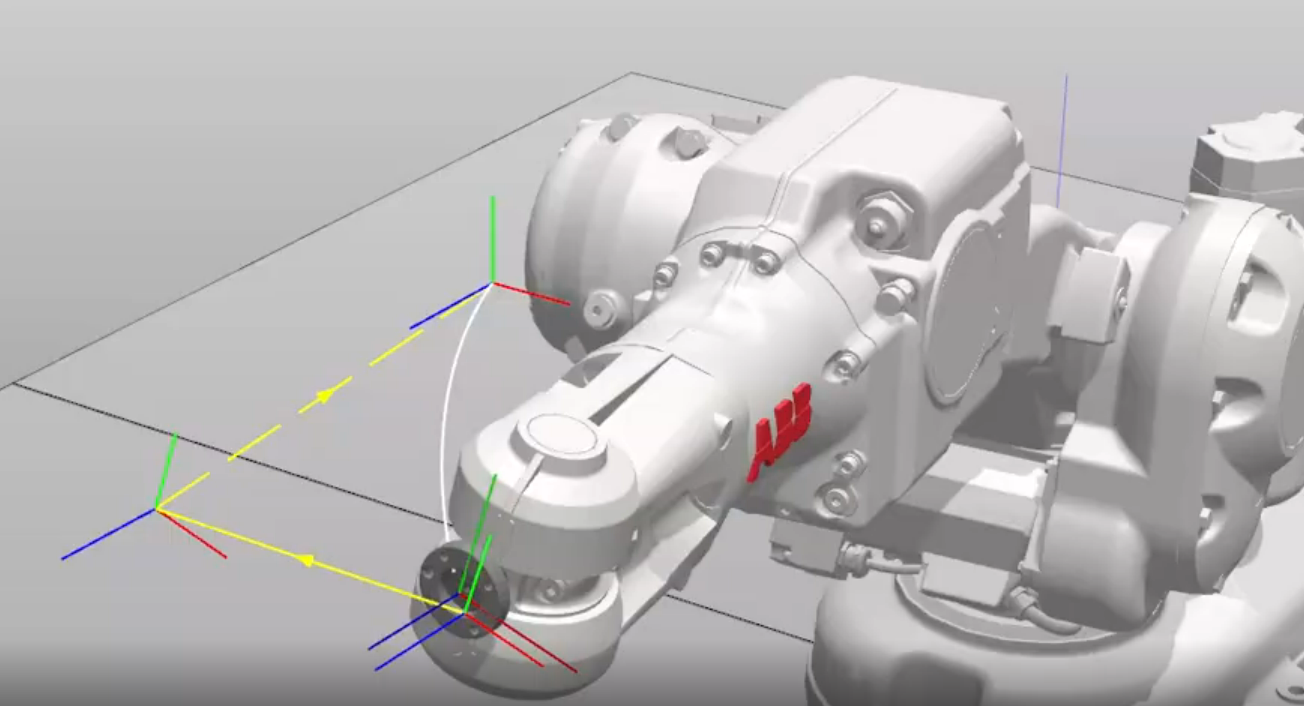
\includegraphics[height=0.75\textheight]{thumbnailhor.png}
		}

		\vspace{0.5em}
		\small Click para reproducir el video
	\end{frame}





	% --- Diapositiva 11: Conclusiones ---
	\begin{frame}{Conclusiones}
		\begin{itemize}
			\item \textbf{Eficacia del método:} El análisis basado en la Jacobiana inversa y la búsqueda por grilla permitió mapear exitosamente el rendimiento cinemático del robot.
			\item \textbf{Identificación del óptimo:} Se logró identificar las regiones del espacio de trabajo donde el manipulador puede desarrollar sus velocidades máximas (brazo extendido).
			\item \textbf{Limitaciones del modelo:} Quedó evidenciada la brecha entre el modelo cinemático ideal de 3 GDL y las restricciones físicas/dinámicas de un sistema de 6 GDL.
		\end{itemize}
	\end{frame}

\end{document}